%%
%% This is file `sample-sigconf-authordraft.tex',
%% generated with the docstrip utility.
%%
%% The original source files were:
%%
%% samples.dtx  (with options: `all,proceedings,bibtex,authordraft')
%% 
%% IMPORTANT NOTICE:
%% 
%% For the copyright see the source file.
%% 
%% Any modified versions of this file must be renamed
%% with new filenames distinct from sample-sigconf-authordraft.tex.
%% 
%% For distribution of the original source see the terms
%% for copying and modification in the file samples.dtx.
%% 
%% This generated file may be distributed as long as the
%% original source files, as listed above, are part of the
%% same distribution. (The sources need not necessarily be
%% in the same archive or directory.)
%%
%%
%% Commands for TeXCount
%TC:macro \cite [option:text,text]
%TC:macro \citep [option:text,text]
%TC:macro \citet [option:text,text]
%TC:envir table 0 1
%TC:envir table* 0 1
%TC:envir tabular [ignore] word
%TC:envir displaymath 0 word
%TC:envir math 0 word
%TC:envir comment 0 0
%%
%%
%% The first command in your LaTeX source must be the \documentclass
%% command.
%%
%% For submission and review of your manuscript please change the
%% command to \documentclass[manuscript, screen, review]{acmart}.
%%
%% When submitting camera ready or to TAPS, please change the command
%% to \documentclass[sigconf]{acmart} or whichever template is required
%% for your publication.
%%
%%
\documentclass[sigconf]{acmart}
\usepackage{hyperref}
\usepackage{enumitem}
\newlist{arrowlist}{itemize}{1}
\setlist[arrowlist]{label=$\Rightarrow$}
%%\usepackage{indentfirst}

%%
%% \BibTeX command to typeset BibTeX logo in the docs
\AtBeginDocument{%
  \providecommand\BibTeX{{%
    Bib\TeX}}}

%% Rights management information.  This information is sent to you
%% when you complete the rights form.  These commands have SAMPLE
%% values in them; it is your responsibility as an author to replace
%% the commands and values with those provided to you when you
%% complete the rights form.
\setcopyright{acmlicensed}
\copyrightyear{2024}
\acmYear{2024}
\acmDOI{}

%% These commands are for a PROCEEDINGS abstract or paper.
\acmConference[G51]{PRI}{October 13, 2024}{Porto, PT}
%%
%%  Uncomment \acmBooktitle if the title of the proceedings is different
%%  from ``Proceedings of ...''!
%%
%%\acmBooktitle{Woodstock '18: ACM Symposium on Neural Gaze Detection,
%%  June 03--05, 2018, Woodstock, NY}
\acmISBN{978-1-4503-XXXX-X/18/06}


%%
%% Submission ID.
%% Use this when submitting an article to a sponsored event. You'll
%% receive a unique submission ID from the organizers
%% of the event, and this ID should be used as the parameter to this command.
%%\acmSubmissionID{123-A56-BU3}

%%
%% For managing citations, it is recommended to use bibliography
%% files in BibTeX format.
%%
%% You can then either use BibTeX with the ACM-Reference-Format style,
%% or BibLaTeX with the acmnumeric or acmauthoryear sytles, that include
%% support for advanced citation of software artefact from the
%% biblatex-software package, also separately available on CTAN.
%%
%% Look at the sample-*-biblatex.tex files for templates showcasing
%% the biblatex styles.
%%

%%
%% The majority of ACM publications use numbered citations and
%% references.  The command \citestyle{authoryear} switches to the
%% "author year" style.
%%
%% If you are preparing content for an event
%% sponsored by ACM SIGGRAPH, you must use the "author year" style of
%% citations and references.
%% Uncommenting
%% the next command will enable that style.
%%\citestyle{acmauthoryear}


%%
%% end of the preamble, start of the body of the document source.
\begin{document}

%%
%% The "title" command has an optional parameter,
%% allowing the author to define a "short title" to be used in page headers.
\title{PRIMED: A Medicine Search System}

%%
%% The "author" command and its associated commands are used to define
%% the authors and their affiliations.
%% Of note is the shared affiliation of the first two authors, and the
%% "authornote" and "authornotemark" commands
%% used to denote shared contribution to the research.
\author{Pedro Simões}
\email{up202403063@up.pt}
\affiliation{%
  \institution{Faculdade de Engenharia da Universidade do Porto}
  \city{Porto}
  \country{Portugal}
}

\author{Miguel Garrido}
\email{up202108889@up.pt}
\affiliation{%
	\institution{Faculdade de Engenharia da Universidade do Porto}
	\city{Porto}
	\country{Portugal}
}

\author{Emanuel Maia}
\email{up202107486@up.pt}
\affiliation{%
	\institution{Faculdade de Engenharia da Universidade do Porto}
	\city{Porto}
	\country{Portugal}
}

\author{Guilherme Martins}
\email{up202403106@up.pt}
\affiliation{%
	\institution{Faculdade de Engenharia da Universidade do Porto}
	\city{Porto}
	\country{Portugal}
}

%%
%% By default, the full list of authors will be used in the page
%% headers. Often, this list is too long, and will overlap
%% other information printed in the page headers. This command allows
%% the author to define a more concise list
%% of authors' names for this purpose.
\renewcommand{\shortauthors}{Pedro Simões, Miguel Garrido, Emanuel Maia and Guilherme Martins}

%%
%% The abstract is a short summary of the work to be presented in the
%% article.
\begin{abstract}
The PRIMED project aims to enhance access to structured pharmaceutical data for healthcare and research by collecting and processing information on medicines, diseases, manufacturers, and user reviews. This paper details the latest milestone, which involves data collection from diverse sources such as Kaggle and Wikipedia, followed by a comprehensive data pipeline implemented in Python. Key steps in this pipeline include data cleaning, text normalization, and standardization of formats, ensuring the data is structured and easily searchable. The model stores data in a JSON format, making it compatible with future integration into larger systems. Preliminary results indicate that the processed data improves accessibility and organization, providing a valuable resource for healthcare professionals and researchers in making informed decisions. \end{abstract}

%%
%% The code below is generated by the tool at http://dl.acm.org/ccs.cfm.
%% Please copy and paste the code instead of the example below.
%%
\begin{CCSXML}
<ccs2012>
   <concept>
       <concept_id>10002951.10003317.10003325</concept_id>
       <concept_desc>Information systems~Information retrieval query processing</concept_desc>
       <concept_significance>100</concept_significance>
       </concept>
 </ccs2012>
\end{CCSXML}

\ccsdesc[100]{Information systems~Information retrieval query processing}

%%
%% Keywords. The author(s) should pick words that accurately describe
%% the work being presented. Separate the keywords with commas.
\keywords{Medicine, Treatments, Sickness, Pipeline, Data, Gathering, Scraping, Preparation, Search Engine}
%% A "teaser" image appears between the author and affiliation
%% information and the body of the document, and typically spans the
%% page.

%%
%% This command processes the author and affiliation and title
%% information and builds the first part of the formatted document.
\maketitle

\section{Introduction}
Nowadays, accurate and comprehensive medicine information plays a vital role in decision-making on the healthcare and investigation sectors. Having access to clean and relevant information is crucial to enhance the efficiency and safety of treatments.

The \textit{\textbf{PRIMED}} project aims to compile and organize such data so that it can be accessed in an easy and organized way. It provides insights that can be applied both in practical cases or simply in developing new health safety politics.

In this part of the project, data from various sources was collected, processed and analysed with the goal of creating a solid basis for a pharmaceutical system. The whole process is described in this document, from the choice of the theme itself up to the analysis of gathered data and its subsequent classification.

\section{Theme Selection}
The choice to focus on medicines as the central theme for this project stems from the critical role they play in modern healthcare. Medication is the primary tool for treating multiple health problems and conditions, making them an essential component in both public healthcare systems and individual patient care. The data surrounding these substances, such as active substances, applicable cases and clinical trials, offers valuable insights that can improve decision-making in medical practice and pharmaceutics.

\section{Data Collection}
This chapter outlines the data selection process and the methods utilized to gather it.

\subsection{Selection of Data}
One of the main challenges of the healthcare sector is ensuring that accurate and up-to-date information on medication is available to healthcare professionals. Given these needs, the selection of data to be collected was made:

\begin{itemize}
	\item {\texttt{Medicines}}: The main component of the data, consisting of medicines and their respective relevant, intrinsic information.
	\item {\texttt{Diseases}}: To complement the collected data, information on some diseases was collected so that it would be possible to get more information to allow for an easier medicine selection process.
	\item {\texttt{Pharmaceutical Companies}}: Some pharmaceutical companies are more trusted than others due to their credibility and higher quality products, which can impact the decision-making process.
	\item {\texttt{Reviews}}: It is important to know the success rate of the presented medicine and how the people who use it feel about it.
\end{itemize}

With this data, the aim is to provide the required information to the users.

\subsection{Gathering}

Finding data suitable for the project proved to be a challenge; not only did it have to be relevant and accurate, but it also had to meet some criteria in terms of quantity and quality. Therefore, the data had to be gathered from multiple sources using different methods - most of the data came from prepared datasets found on Kaggle\cite{kaggle}, while the rest came from scraping Wikipedia\cite{wikipedia}.

\subsubsection{Medicines}

The \textit{Medicines} dataset\cite{medicines_dataset}, retrieved from Kaggle, contains a list of pharmaceutical treatments and some relevant, mostly textual, information about the cases where it is used.

The present information on this dataset is:
\begin{itemize}
	\item {\texttt{Medicine Name}}: The name of the medicine.
	\item {\texttt{Composition}}: The active substance present in the medicine.
	\item {\texttt{Uses}}: A list of cases where the medicine is used (specific diseases, for example).
	\item {\texttt{Side Effects}}: Lists possible side effects resulting from the medicine's usage.
	\item {\texttt{Manufacturer}}: The name of the company responsible for producing the medicine.
	\item {\texttt{Reviews}}: Three additional columns containing the percentage of "Excellent", "Average" and "Poor" reviews for each medicine's treatment results.
\end{itemize}

This dataset, which contains 11824 different medicines, possesses a {\textit{\textbf{CC0 1.0 Universal}}}\cite{cczero} license, which means the data is part of the public domain, allowing for the copying and modification of the data.

\subsubsection{Diseases}

This dataset was scraped from the tables of a Wikipedia page containing a list of autoimmune diseases\cite{diseases_dataset}; by gathering this data, the goal was to complement the previous dataset's "Uses" and "Side Effects" columns by collecting more information on this specific subset of diseases.

The information extracted from this dataset consists of:
\begin{itemize}
	\item {\texttt{Disease}}: The name of the disease.
	\item {\texttt{Primary Organ/Body Part Affected}}: Information on the organs or body parts affected by the disease.
	\item {\texttt{Autoantibodies}}: The antibodies associated with each specific disease.
	\item {\texttt{Acceptance as an Autoimmune Disease}}: Classification for each disease related to its acceptance as an autoimmune condition, based on the current scientific consensus and level of evidence supporting its autoimmune nature.
	\item {\texttt{Prevalence Rate (US)}}: The percentage of people affected by the disease in the United States of America.
\end{itemize}

The gathered dataset contains about 110 lines of diseases, being available under the \textit{\textbf{Creative Commons Attribution-ShareAlike 4.0 International}}\cite{wikipedia_cc} license, which allows for the sharing and adaptation of the contents.

\subsubsection{Pharmaceutical Companies}

To complement the data on companies present in the \textit{Medicines} dataset, more data on pharmaceutical companies was gathered through another round Wikipedia scraping - this time from a page containing an extensive list of pharmaceutical companies\cite{companies_dataset}. Approximately 700 companies' names and founding dates were gathered, alongside a short description from each one's Wikipedia article.

The collected information follows this structure:
\begin{itemize}
	\item {\texttt{Company Name}}: The company's name.
	\item {\texttt{Year}}: The year the company was created and, if available, when the company was shut down.
	\item {\texttt{Description}}: A short description of each company, its values and some extra information.
\end{itemize}

This dataset falls under the same license as the previous \textit{Diseases} dataset (\textit{\textbf{Creative Commons Attribution-ShareAlike 4.0 International}}), as the data was collected in a similar way.

\subsubsection{Reviews}

Lastly, a dataset containing reviews for the collected medication data with more personal descriptions from users\cite{reviews_dataset} was retrieved from UC Irvine's Machine Learning Repository\cite{irvine}.

The data collected had the following structure:
\begin{itemize}
	\item {\texttt{Unique ID}}: The unique identification of the review.
	\item {\texttt{Drug Name}}: Name of the drug/treatment.
	\item {\texttt{Condition}}: The condition of the patient where it was used.
	\item {\texttt{Review}}: Written review of the experience of taking the drug.
	\item {\texttt{Rating}}: Number from 0-10 that expresses the quality of the drug.
    \item {\texttt{Date}}: Date of when the drug was taken.
    \item {\texttt{Useful Count}}: Similar to a "like" system, this showcases the number of people who found this review useful.
\end{itemize}

Each review can only be associated with a single condition/disease, which is a limitation of the dataset itself.

This dataset contains around 215000 entries and is covered by the \textit{\textbf{Attribution 4.0 International}}\cite{ccfour} license, which allows for the sharing and adaptation of the datasets for any purpose, provided that the appropriate credit is given.

\section{Pipeline Description}

As mentioned in section 3.2 of this report, \textit{\textbf{PRIMED}}'s data comes from various sources. Due to the often unstructured nature of this data, it is vital to have a streamlined and automated way of normalizing and processing all the information into similar formats, which is the main role of the data pipeline, present in figure [1].

\begin{figure}[h]
	\centering
	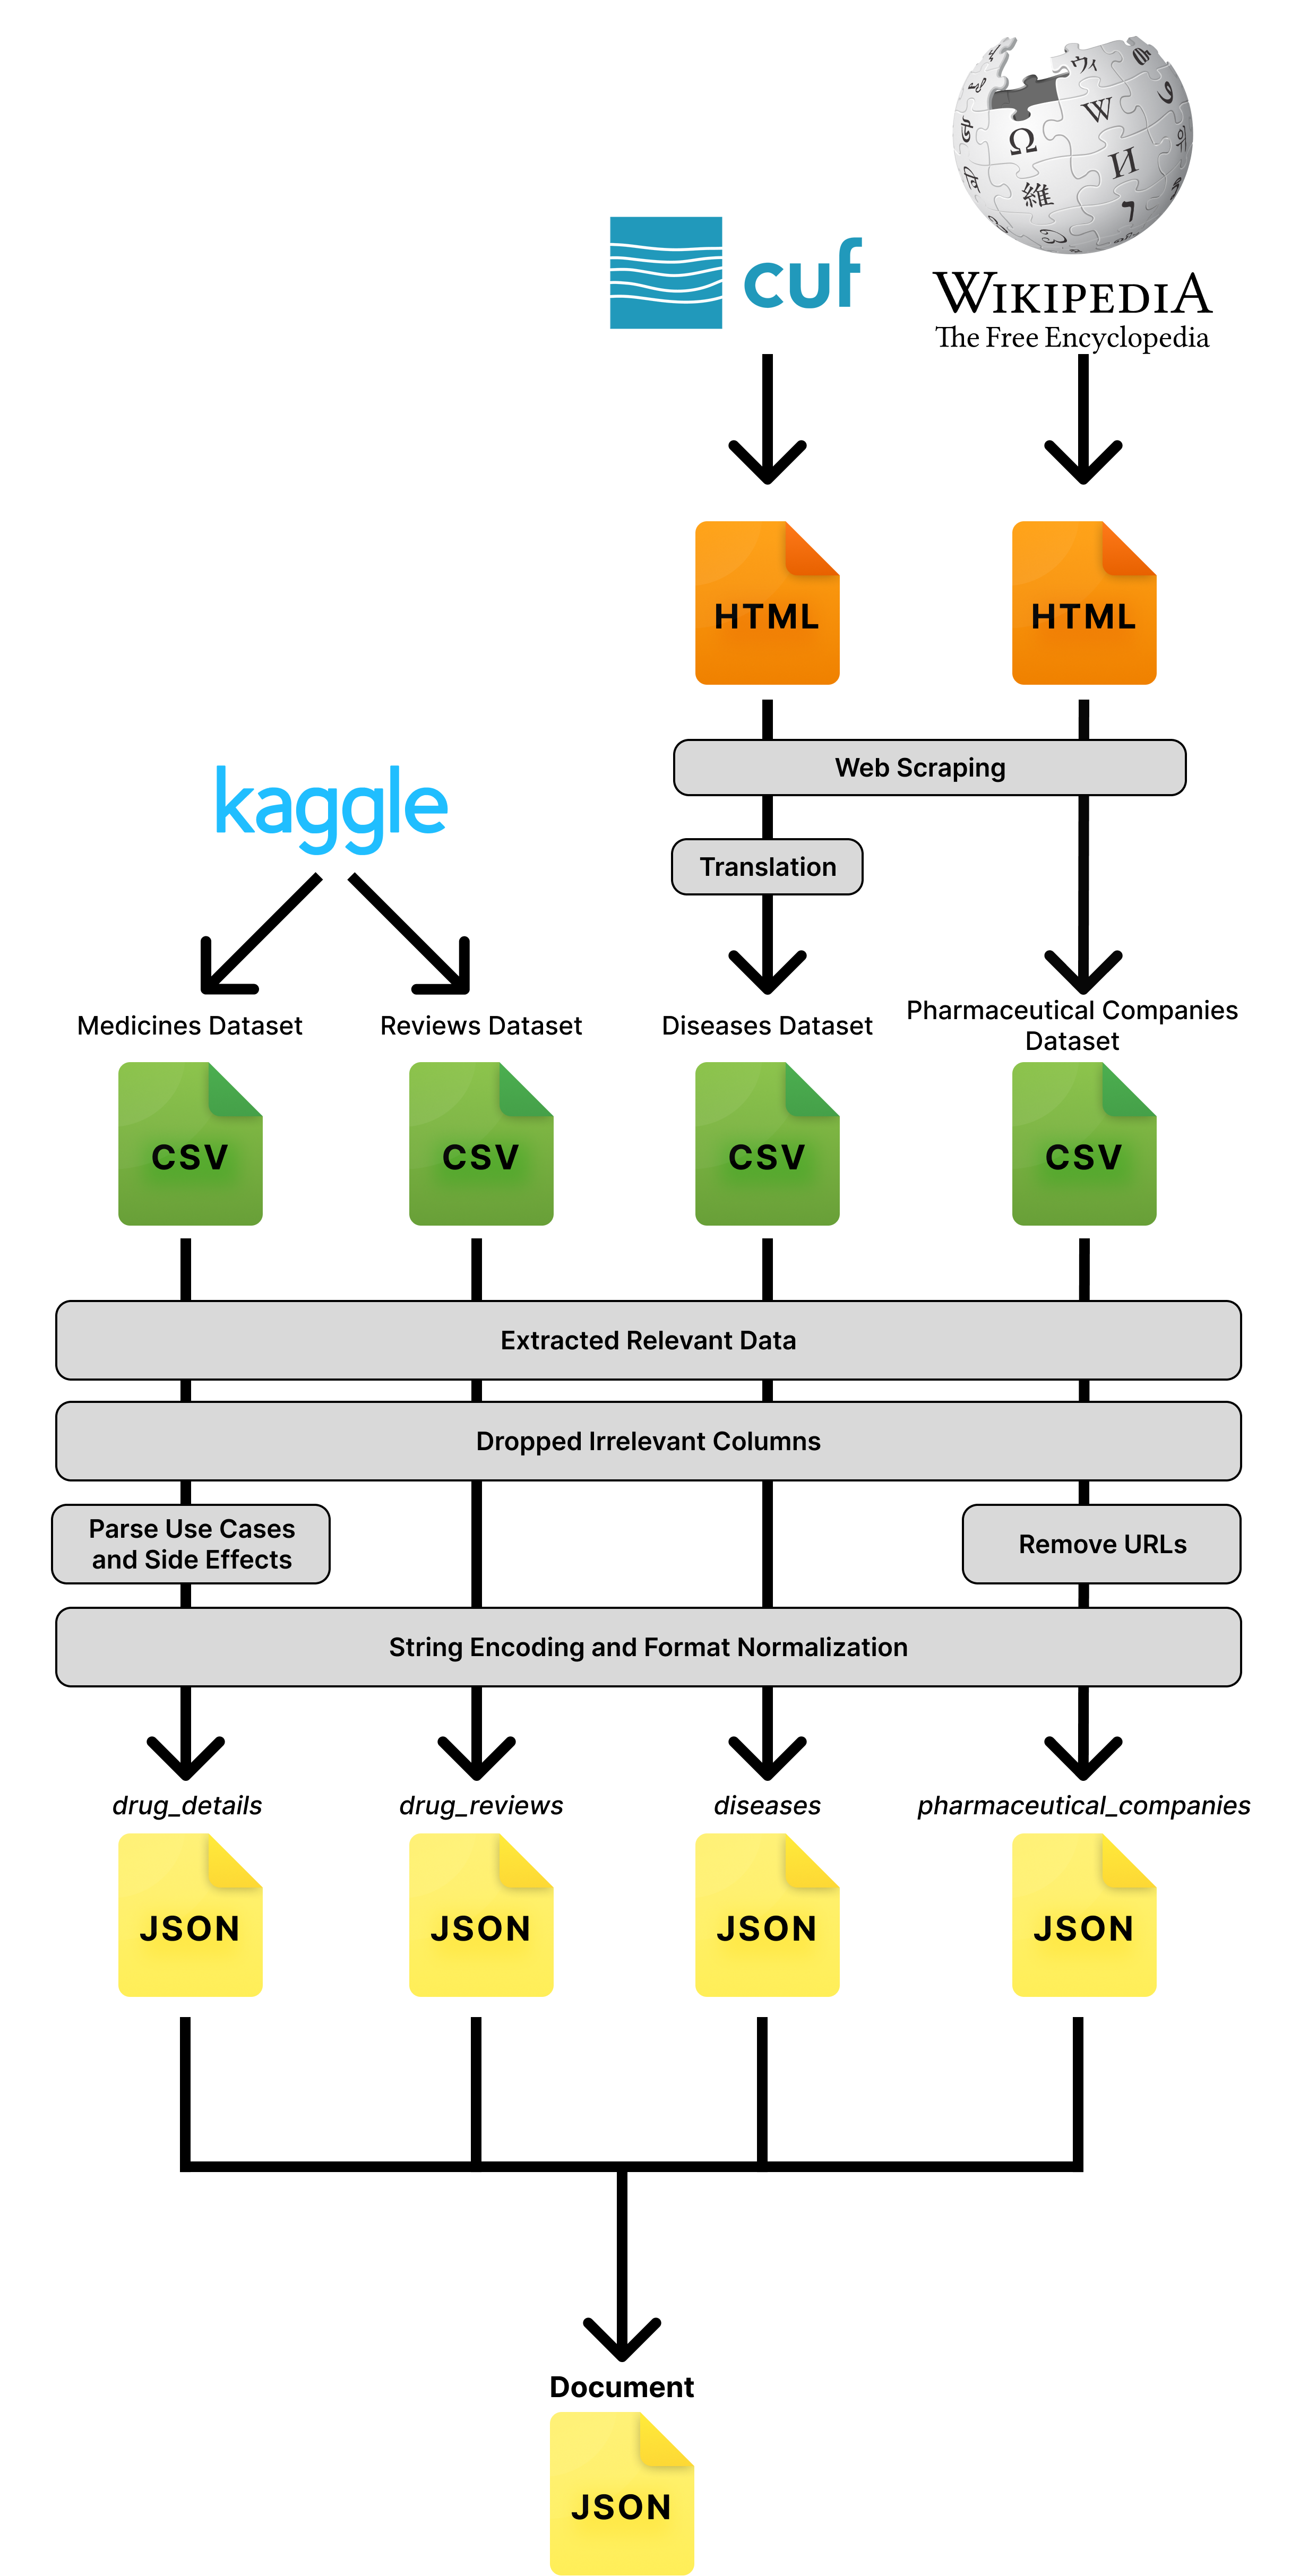
\includegraphics[width=\linewidth]{data_pipeline.png}
	\caption{Data Pipeline}
	\Description{Data Pipeline}
	\label{fig:pipeline}
  \end{figure}

The pipeline consists of \texttt{Python}\cite{python} scripts utilizing libraries such as \texttt{pandas}\cite{pandas}, \texttt{unidecode}\cite{unidecode}, \texttt{html}\cite{html}, \texttt{json}\cite{json} and \texttt{csv}\cite{csv} with the crux of the data processing occurring on the \texttt{to{\textunderscore}json.py} script, which converts the \texttt{CSV} files into \texttt{JSON} format.

\subsection{Elimination of Null Values and Rows}

When processing data, another key aspect to consider is that not all data may be correct or even present. For this reason, before doing anything else with the \texttt{CSV} source files, the pipeline uses \texttt{pandas} \textit{dataframes} to check for and remove rows containing only null values, or rows in which key values, such as \texttt{Medicine Name}, for instance, aren't present.

\subsection{Text Normalization}

When scraping information from websites, it is important to make sure all the text is normalized. The data pipeline ensures, via \texttt{Python}'s \texttt{unidecode()} function, that the dataset only contains \texttt{ASCII} characters. This helps prevent future issues when searching the datasets for information.

Another character normalization problem resulting from the scraping process arises due to \texttt{HTML}'s nature - more specifically, escape codes used to represent special characters. To convert these codes into ASCII characters, the \texttt{unescape()}\cite{html} function from \texttt{Python}'s \texttt{html} module, wrapped inside a call to the previously mentioned \texttt{unidecode()} function, to convert the \texttt{Unicode} output into \texttt{ASCII}.

\subsection{Standardization of Formats}

For the best possible result, formats such as dates should be standardized; therefore, part of the pipeline deals with transforming this data into \texttt{yyyy-mm-dd} format, which makes the process of sorting and searching substantially easier. 

\subsection{Data Storage}

The final output of the pipeline (the processed data that the search engine will be working with) is stored in \texttt{JSON} format. This decision stems from the requirement of a document-based data storage model, where each \texttt{JSON} object represents a document encapsulating all the relevant fields and values for a particular record - in this case, a specific medicine. This approach provides flexibility in handling unstructured data, since there are no hard constraints in place.

This model also ensures the search engine can query and retrieve data efficiently, based on specific fields within these documents, ensuring that the system can scale as the dataset grows; it also supports complex data relationships and makes it easier to analyse information across different records.

\section{Conceptual Data Model}

Having finalized the data collection and the subsequent transformation and storage processes in the pipeline, a conceptual data model for the combined dataset was developed.

\begin{figure}[H]
  \centering
  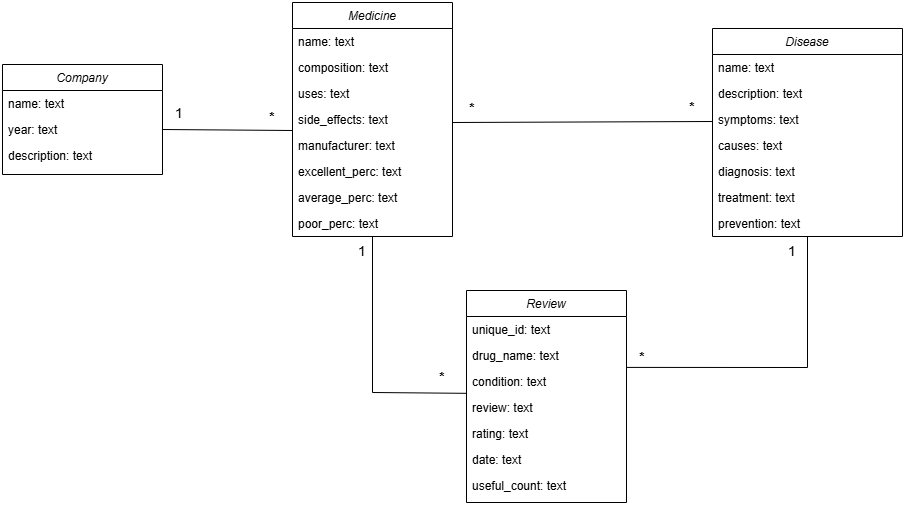
\includegraphics[width=\linewidth]{../pri_uml_final.png}
  \caption{Conceptual Data Model}
  \Description{UML diagram for \textit{\textbf{PRIMED}}'s data}
  \label{fig:uml}
\end{figure}

Each medicine is associated with one and only one pharmaceutical company; a company, however, can produce multiple medicines. A single medicine can be linked to multiple diseases and reviews, though the reverse is true only for diseases - a disease can be associated to many medicines (and many reviews). A review, however, can only be associated with a single medicine and a single disease.

\section{Dataset Characterization}

With regard to the characterization of the dataset, the data resulting from the pipeline was analysed. Graphs, tables and even word clouds, despite not being the most reliable method, were created to make it easier to understand the structure of the data and the patterns that guide the system itself.

\subsection{Distribution of Drug Manufacturers}

By analysing figure [3], which shows the distribution of the main pharmaceutical companies responsible for manufacturing medicines where the five that possess the largest share are highlighted, we are given a clearer understanding of each manufacturers' production capabilities.

\subsection{Distribution of Reviews}

A box plot, present in figure [4], is utilized to analyse the distribution of “Excellent”, “Average” and “Poor” review percentages across the different medicines. The graph shows that, for instance, "Excellent" reviews percentages are more evenly spread than the "Average" reviews percentages which, despite having a lower interquartile range\cite{iqrange}, possesses a higher number of outliers. The "Poor" review percentages have the largest variations, but also the lowest values. 

In figure [5], we can see the average percentage of reviews for the top ten use cases, which supports the findings from figure [4].

\subsection{Distribution of Side Effects}

By analysing figure [6], we can identify the most common side effects caused by medication - nausea, headaches, diarrhea - and how many medicines are associated to each one of them. As expected, the data shows that side effects that occur more frequently are those that are milder in nature.

\subsection{Common Uses Word Cloud}

Figure [7] contains a word cloud with the most common use cases for medicines. “Bacterial Infections” and "Hypertension", for example, are clearly highlighted in the graph, being conditions that are found and treated more frequently.

\subsection{Most Common Drug Compositions}

Figure [8] identifies the the most common drug combinations available in the market, with “Levocetirizine + Montelukast” being the most prevalent, followed by other combinations such as “Luliconazole” and “Domperidone + Rabeprazole”.

\subsection{Years with the Most Companies Foundations}	

By analysing figure [9], it's possible to observe the years in which the most pharmaceutical companies were founded, with 2003 standing out. This temporal analysis gives us some information about periods of significant growth in the pharmaceutical industry.

\subsection{General description}

The final dataset contains 11498 entries, each one representing a drug with all information related to it. The present info on the drug are reviews, their text and usefulness, the manufacturer and it's details, diseases and more text info about each of them and the previously discussed drug information.

\section{Information Needs}

The information needs can vary depending on the person using \textit{\textbf{PRIMED}}. If the individual who is using the tool is, for example, a doctor or a pharmacist, these needs might be related to the compositions of a medicine or cases where it can be applied. If the user is a patient (an average person), they might be more interested in checking which company manufactures the medicine to check if it can be trusted or to assess other user's reviews of that treatment, as well as possible side effects, to have a better understanding of what can happen to them.

Here is a list of possible information needs, explaining what type of data is needed, why and for whom:
\begin{itemize}
	\item {\texttt{Medicine Compositions}}: The composition of medication is an important aspect since some might be harmful to the patient, depending on what kind of active substances are present.
	\item {\texttt{Uses}}: Not every medicine has clearly defined use cases; some may have a primary use while also being beneficial for other less common conditions.
	\item {\texttt{Side Effects}}: The users should be aware of possible side effects resulting from their treatment, so that they can be informed and prepared for potential symptoms or strange events.
	\item {\texttt{Manufacturer}}: Some people have a preference for specific manufacturers who they trust more than others, or can simply want to gather more information on the company producing the medicine they were prescribed.
	\item {\texttt{Reviews}}: For all possible types of users, existing reviews are always important - whether they are textual or not. These indicate other people's experiences with a particular medicine and can even report some peculiar cases where the patients experienced rare effects from that treatment.
	\item {\texttt{Diseases' Primary Organs/Autoantibodies}}: In some cases, experts might need to know what part of the body or organs are most affected by a disease, or what antibodies are linked to it, in order to prescribe the best solution.
	\item {\texttt{Prevalence Rate}}: It can also be relevant to be aware of how common a certain disease is in a population, whether that influences the diagnosis of the patient or just for statistical purposes.
\end{itemize}

Based one these needs, we can answer some questions like: 
\begin{arrowlist}
	\item Which medicines are more commonly used to treat the common cold?
    \item Trustworthy companies that provide medicines for Alzheimer’s disease. 
	\item How does the composition of medicine for diabetes vary between manufacturers like Novo Nordisk, Eli Lilly, and Sanofi?
	\item What are the most effective treatments for managing rheumatoid vasculitis pain and inflammation?
	\item What is the best treatment for persistent migraine symptoms, including nausea and light sensitivity?
	\item Is weight gain a common side effect of antidepressants?
	\item What side effects have other patients experienced with medications like rituximab or methotrexate for treating vasculitis?
\end{arrowlist}

As previously stated, a wide range of people can take advantage of this type of information - from regular patients to medicine experts and even investigators, everyone can benefit from having access to the data present in \textit{\textbf{PRIMED}}.

\section{Dataset Characterization}

With regard to the characterization of the dataset, the data resulting from the pipeline was analysed. Graphs, tables and even word clouds, despite not being the most reliable method, were created to make it easier to understand the structure of the data and the patterns that guide the system itself.

\subsection{Distribution of Drug Manufacturers}

By analysing figure [3], which shows the distribution of the main pharmaceutical companies responsible for manufacturing medicines where the five that possess the largest share are highlighted, we are given a clearer understanding of each manufacturers' production capabilities.

\subsection{Distribution of Reviews}

A box plot, present in figure [4], is utilized to analyse the distribution of “Excellent”, “Average” and “Poor” review percentages across the different medicines. The graph shows that, for instance, "Excellent" reviews percentages are more evenly spread than the "Average" reviews percentages which, despite having a lower interquartile range\cite{iqrange}, possesses a higher number of outliers. The "Poor" review percentages have the largest variations, but also the lowest values. 

In figure [5], we can see the average percentage of reviews for the top ten use cases, which supports the findings from figure [4].

\subsection{Distribution of Side Effects}

By analysing figure [6], we get to know what are the most common side effects caused by medication - nausea, headaches, diarrhea - and how many medicines are associated to each one of them. As expected, the data shows that side effects that arise more frequently are those that are more mild in nature.

\subsection{Common Uses Word Cloud}

Figure [7] contains a word cloud with the most common use cases for medicines. “Bacterial Infections” and "Hypertension", for example, are clearly highlighted in the graph, being conditions that are found and treated more frequently.

\subsection{Most Common Drug Compositions}

In figure [8], the pie chart shows the five most common drug combinations. The combination “Levocetirizine + Montelukast” is the most frequent, followed by other combinations such as “Luliconazole” and “Domperidone + Rabeprazole”. This visualization makes it easier to identify the most popular compositions for treating diseases.

\subsection{Years with the Most Companies Foundations}	

In figure [9], we can see the years in which the most pharmaceutical companies were founded. 2003 is the year in which the most companies were founded. This temporal analysis helps us to understand the periods of greatest growth in the pharmaceutical industry.

\section{Results}

Having completed this milestone of the project marks a very important step in the development of our system. The work carried out to this date has made it possible to transform an initial set of diverse, loosely related data into a cohesive and structured basis for \textit{\textbf{PRIMED}}. By carrying out data cleaning operations, we have been able to maintain the quality of the information while simultaneously reducing inconsistencies and duplicates. Outfitted with this data, \textit{\textbf{PRIMED}} will be able to offer users a practical source for consulting medical information; however, we will keep an eye on the dataset in case there is a need for further enhancements during future milestones.

\section{System Overview}
Apache SOLR is a search and analysis platform which allows the indexation of big data volumes and to make quick and efficient queries on that data. The way it works is by making the indexation of documents and then creating an efficient association of words and the documents they appear on. With that, the queries made are faster because when the user searches for a word, SOLR checks the index.\cite{solr} SOLR also allows the usage of other "tools" such as boosters to enhance the querying process and others like fuzziness to try and correct typos on the queries.

\subsection{Objectives}
The objectives with SOLR are to create a way to find and access information with quickness and ease, allowing for easy queries with fast results and some enhancement to them. We are also using this opportunity to enhance our documents, adding more text information and changing the numbered values to more meaningful ones.

\subsection{System Architecture}

\section{Final Document}
Here the final document is described and analysed, having some other relevant information related to it considered.

\subsection{Document Definition}
The final document consists of the following field types:
\begin{itemize}
	\item {\texttt{Drug}}: The name of the drug in question.
	\item {\texttt{Composition}}: Composition of the drug.
	\item {\texttt{Applicable diseases}}: List of diseases where the drug is normally applied.
	\item {\texttt{Diseases information}}: Also a list of information about the diseases specified before.
	\item {\texttt{Possible side effects}}: List of possible side effects of the drug when taken.
	\item {\texttt{Excellent review percentage}}: Percentage 
\end{itemize}

\appendix
\section{Annexes}

\begin{figure}[H]
	\centering
	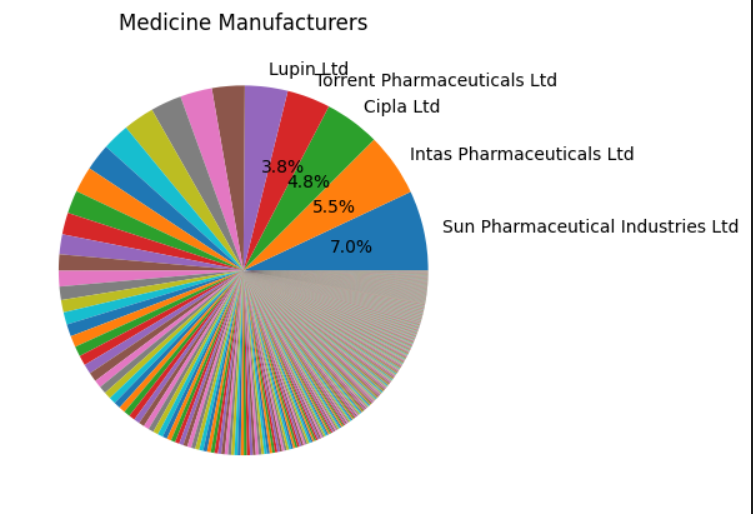
\includegraphics[width=\linewidth]{graphic1.png}
	\caption{Top Drug Manufacturers}
	\Description{Dataset Characterization \textit{\textbf{PRIMED}}'s data}
	\label{fig:uml}
  \end{figure}

\begin{figure}[H]
	\centering
	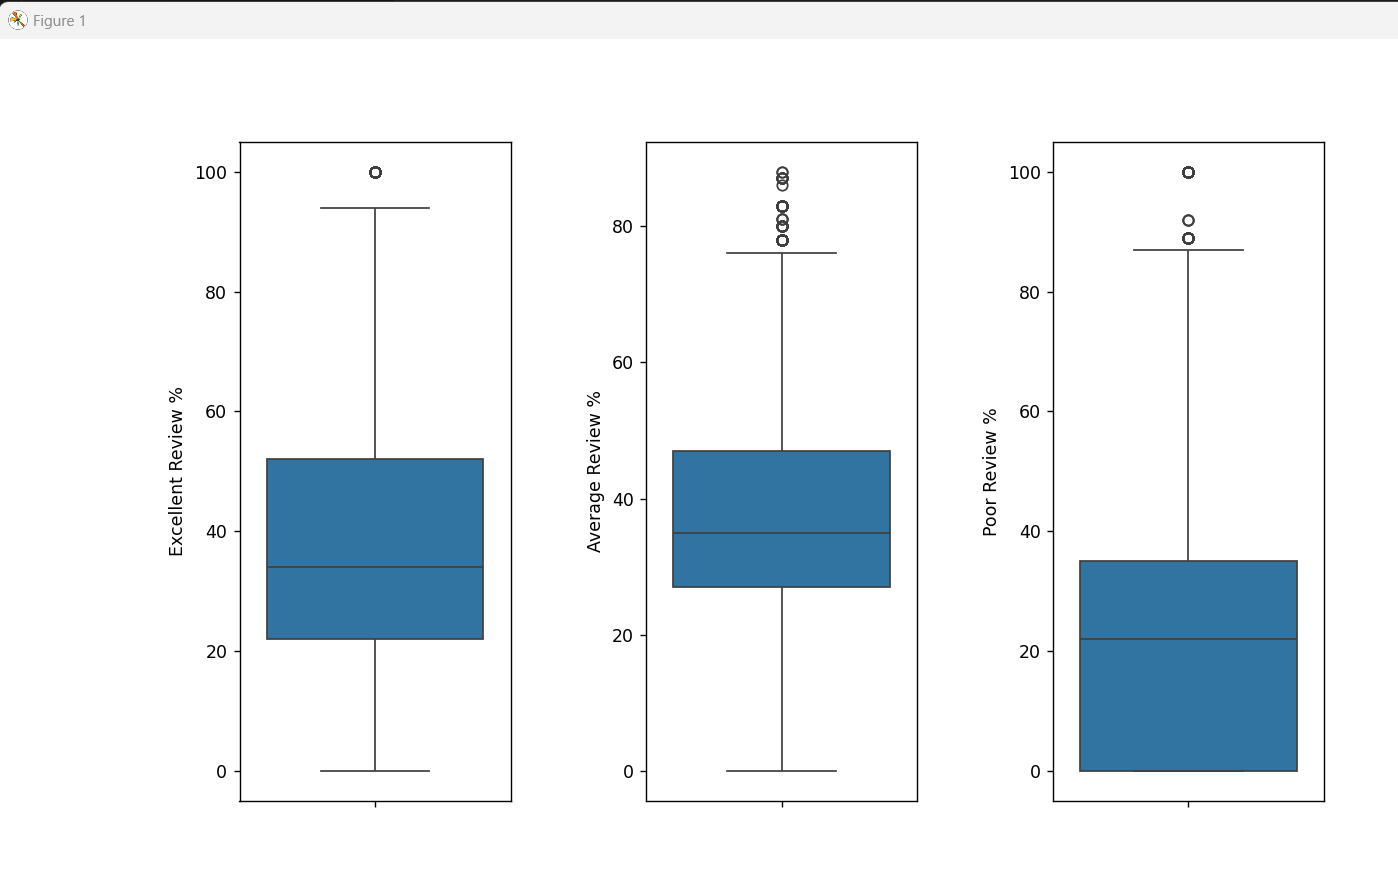
\includegraphics[width=\linewidth]{graphic2.png}
	\caption{Distribution of Reviews}
	\Description{Dataset Characterization \textit{\textbf{PRIMED}}'s data}
	\label{fig:uml}
  \end{figure}

\begin{figure}[H]
	\centering
	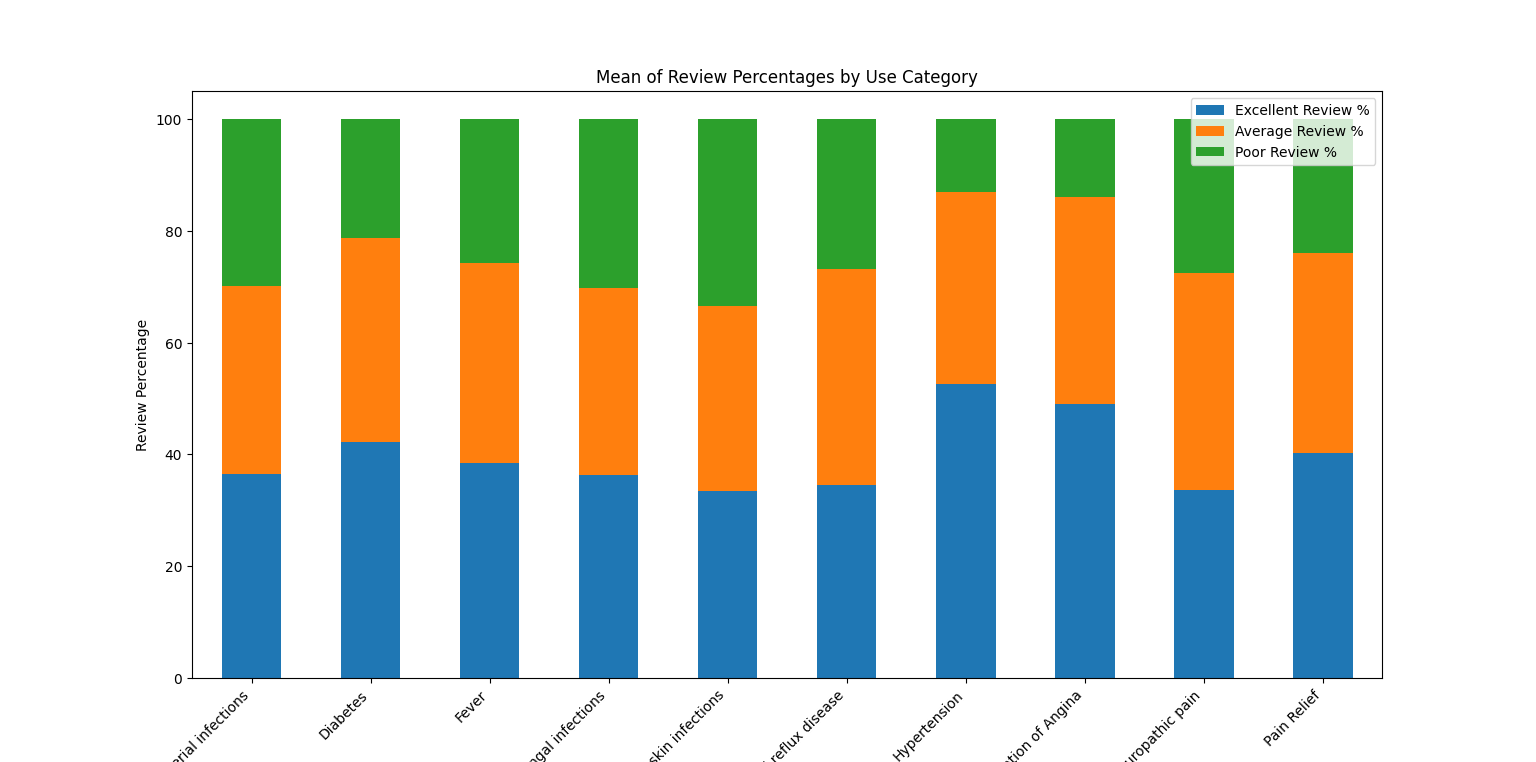
\includegraphics[width=\linewidth]{graphic3.png}
	\caption{Mean of Reviews Percentages by Uses}
	\Description{Dataset Characterization \textit{\textbf{PRIMED}}'s data}
	\label{fig:uml}
  \end{figure}

\begin{figure}[H]
	\centering
	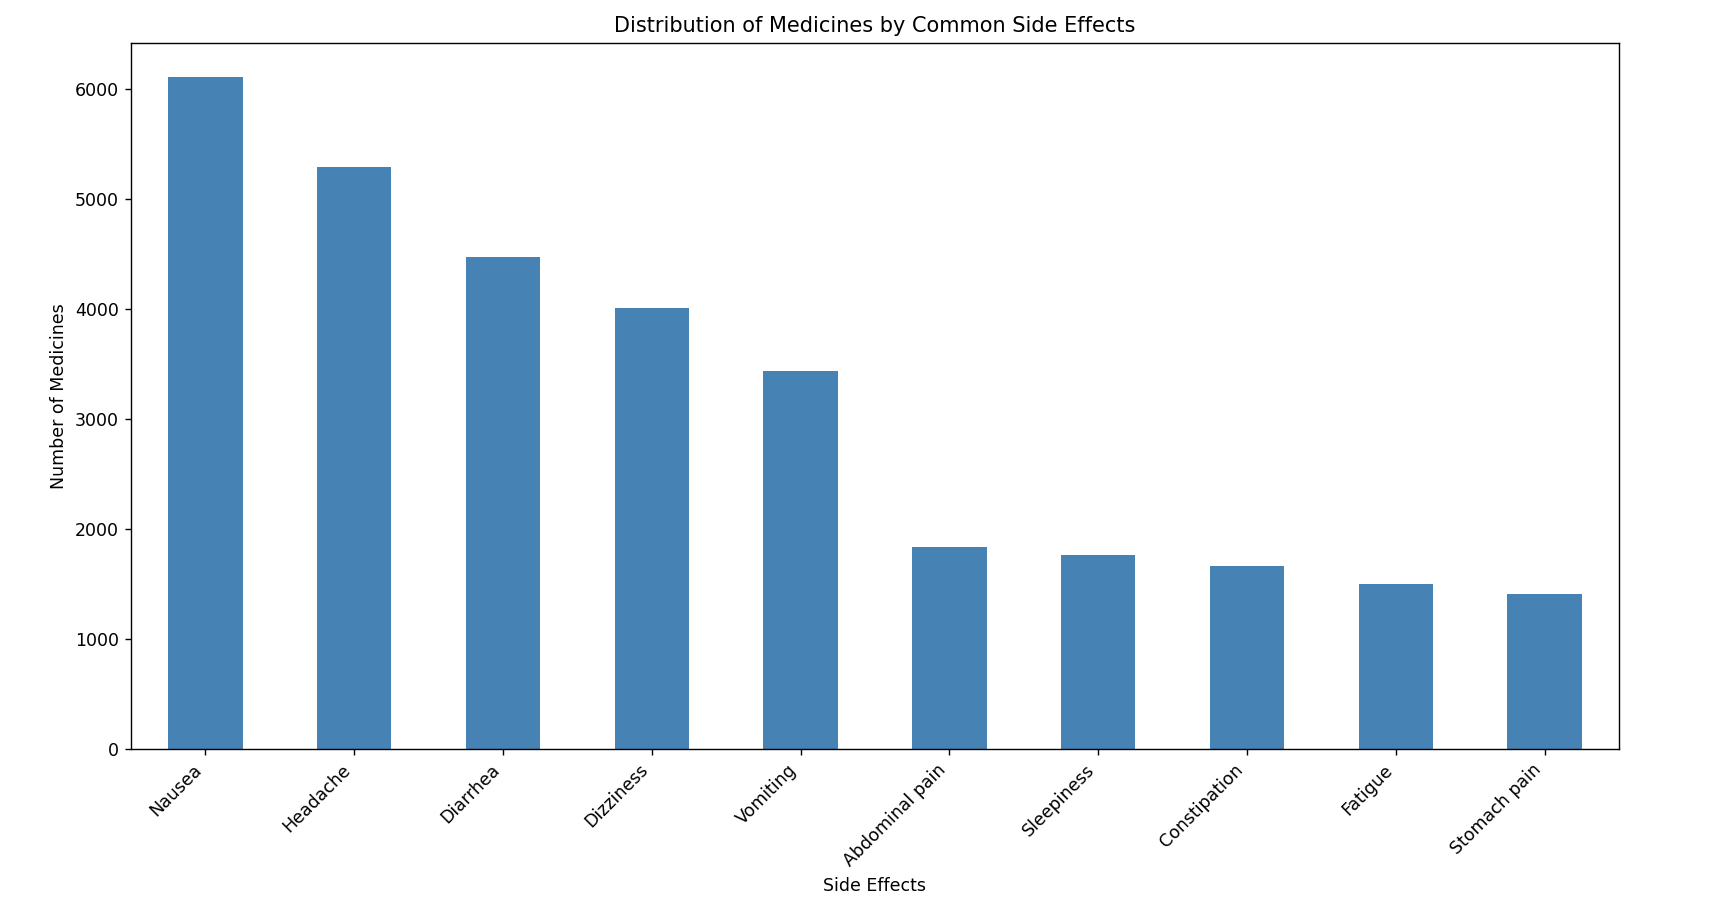
\includegraphics[width=\linewidth]{graphic4.png}
	\caption{Distribution of Side Effects}
	\Description{Dataset Characterization \textit{\textbf{PRIMED}}'s data}
	\label{fig:uml}
  \end{figure}

\begin{figure}[H]
	\centering
	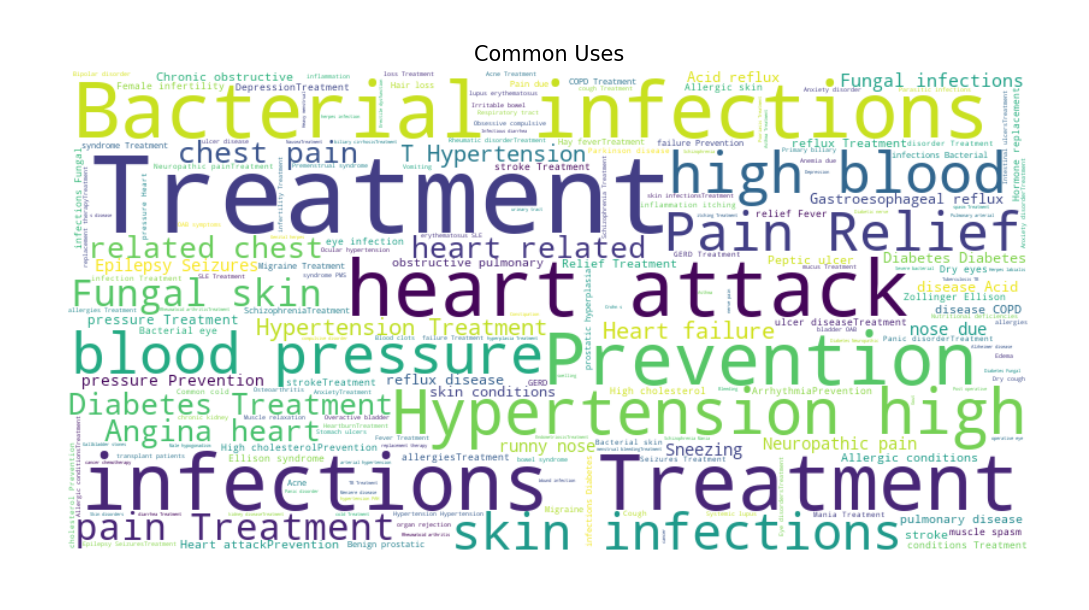
\includegraphics[width=\linewidth]{graphic5.png}
	\caption{Common Uses Word Cloud}
	\Description{Dataset Characterization \textit{\textbf{PRIMED}}'s data}
	\label{fig:uml}
  \end{figure} 

\begin{figure}[H]
	\centering
	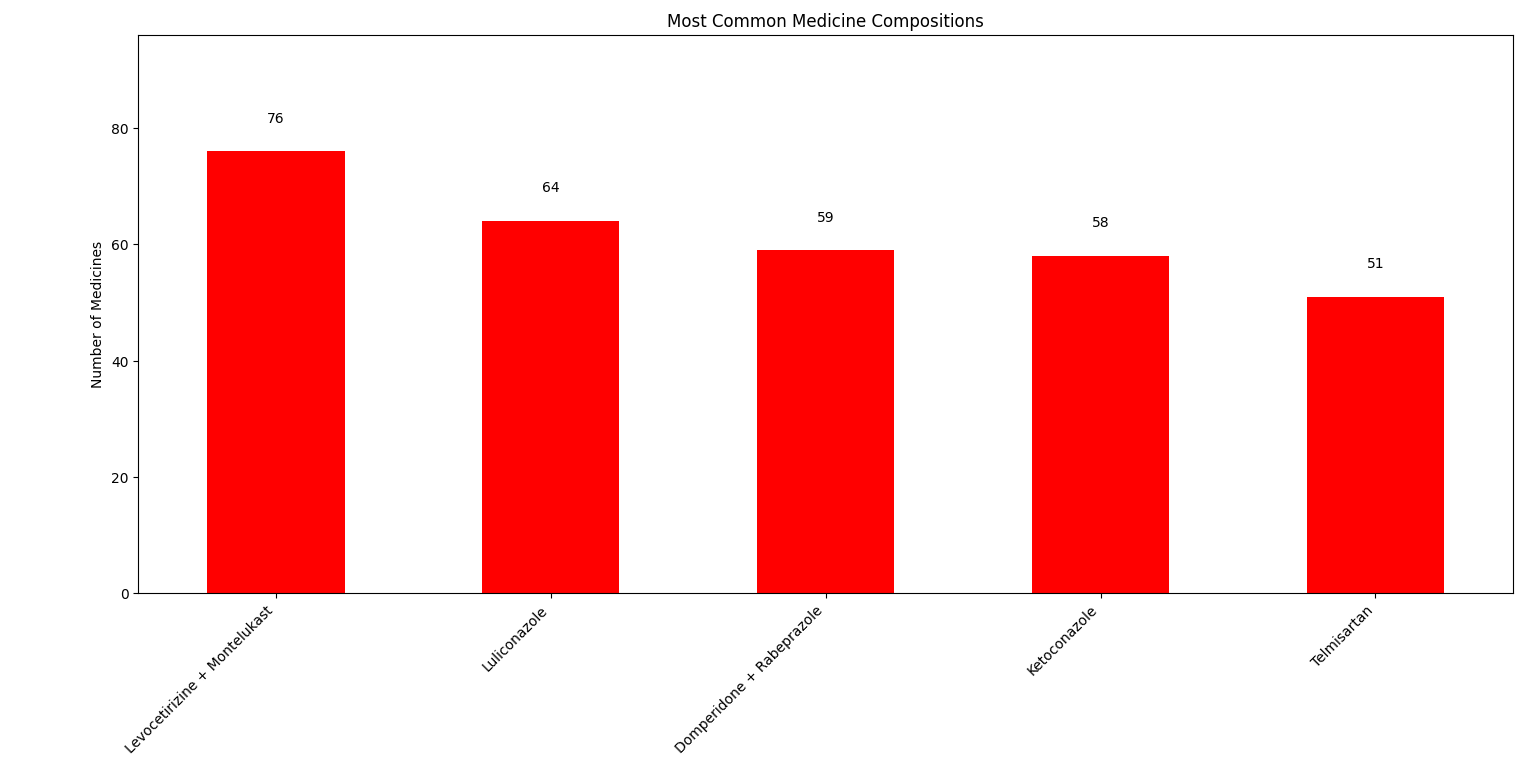
\includegraphics[width=\linewidth]{graphic6.png}
	\caption{Most Common Drug Compositions}
	\Description{Dataset Characterization \textit{\textbf{PRIMED}}'s data}
	\label{fig:uml}
  \end{figure}   

\begin{figure}[H]
	\centering
	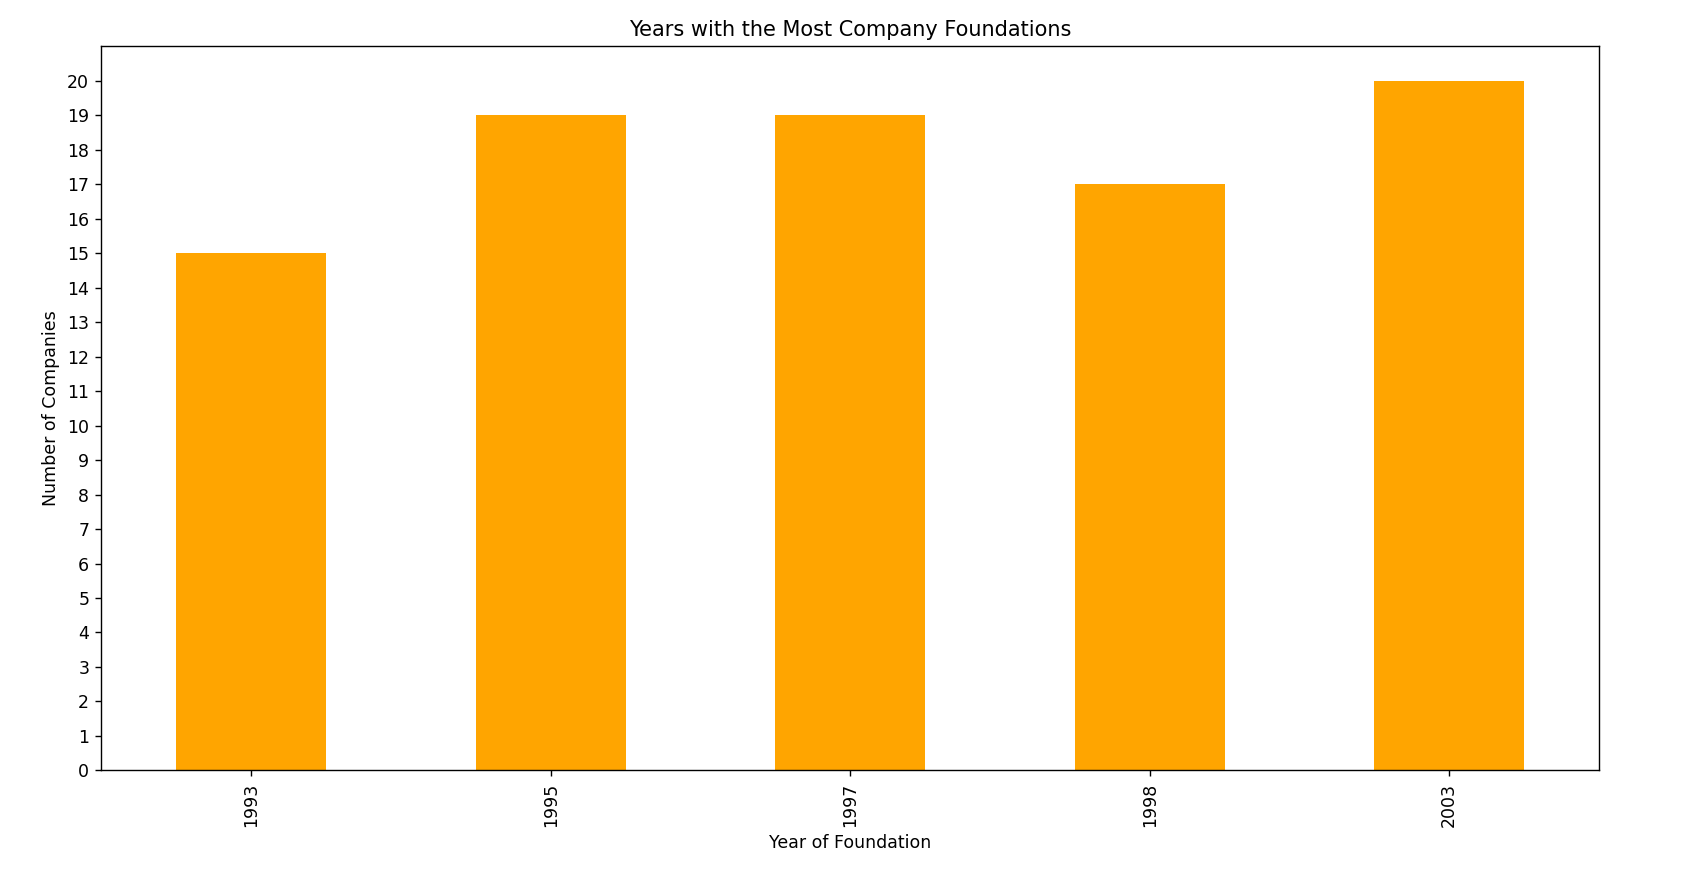
\includegraphics[width=\linewidth]{graphic7.png}
	\caption{Years with the Most Companies Foundations}
	\Description{Dataset Characterization \textit{\textbf{PRIMED}}'s data}
	\label{fig:uml}
  \end{figure}

%%
%% The next two lines define the bibliography style to be used, and
%% the bibliography file.
%%\bibliographystyle{ACM-Reference-Format}
\bibliographystyle{unsrt}
\bibliography{sample-base}


%%
%% If your work has an appendix, this is the place to put it.
%%\appendix

\end{document}
\endinput
%%
%% End of file `sample-sigconf-authordraft.tex'.
